\documentclass[11pt]{article}

%% Escrevendo em português
\usepackage[brazil]{babel}
\usepackage[utf8]{inputenc}
\usepackage[usenames,dvipsnames,svgnames,table]{xcolor}
\usepackage[a4paper,margin={1in}]{geometry}
\usepackage{graphicx}
\usepackage[export]{adjustbox}
\usepackage{color}

%% Pulando linhas
\renewcommand{\baselinestretch}{1.5}

\newcommand{\vsp}{\vspace{0.2in}}
\newcommand{\hsp}{\hspace{1cm}}

\begin {document}



  \begin{minipage}[t]{5in}
    \begin{center}
    {\Large \bf Relatório do projeto - MAC 444\\}
    {\small Profa. Renata Wassermann}
    \end{center}
  \end{minipage}

\vsp \vsp


\section{Integrantes}

\begin{tabular}{ll}
\textbf {Nome} &  \textbf {NUSP} \\
Adnan Yulji Degaki & 7991110 \\
Carlos Eduardo Leão Elmadjian & 5685741 \\
\end{tabular}

\vsp

%============================================================

\section{Arquivos}

\begin{itemize}
	\item \textbf{Relatorio.pdf} -- relatório do projeto;
	\item \textbf{script.py} -- script utilizado para gerar indivíduos na ontologia no formato OWL;
	\item \textbf{ontologia.owl} -- arquivo OWL com a ontologia do projeto.
\end{itemize}

\vsp

%============================================================

\section{Ontologia}
	Nossa ontologia foi construída levando em conta não só as orientações, mas também as sugestões do enunciado do projeto. Nos inspiramos fortemente na \textit{Computer Science Department Ontology}, disponível em um repositório da Universidade de Maryland e recomendada nas instruções do projeto.
	
	Além dos conceitos exigidos, outros como \textit{País}, \textit{Continente} ou \textit{Artigo em Revista} foram adicionados tendo em vista a necessidade de atender adequadamente as requisições em SPARQL. Conceitos além do escopo minimal foram abandonados, tanto porque traziam consigo um acréscimo de complexidade significativo na automatização e incompatível com as necessidades, como também pela dificuldade em mapear corretamente dados ambíguos gerados pelo \textit{scriptlattes} em nosso script para população dos indivíduos.
	
	A ontologia foi construída a partir do arquivo FOAF-modified.rdf, disponibilizado no \textit{site} do projeto. Por \textit{compliance}, as propriedades e conceitos requeridos foram mantidos na versão final, mas nem todos foram utilizados na nossa ontologia. Além disso, elementos adicionais e dispensáveis foram removidos para facilitar a manipulação e a compreensão da ontologia. Alguns detalhes intrínsecos à formatação, como os caminhos IRI, foram padronizados para que houvesse uma maior consistência de dados e as consultas SPARQL fossem facilitadas.
	
	Alguns conceitos exigidos tinham um grau de ambiguidade, como \textit{Aluno}. Nesses casos, definimos critérios próprios para empobrecer um pouco a semântica e tornar nosso trabalho viável. Casos específicos são explicados com mais detalhes na seção de \textbf{consultas SPARQL}.
	
	\subsection{Estrutura de classes}
		Após as modificações relatadas na seção anterior, a estrutura de classes criada segue abaixo:
		
		\begin{center}
			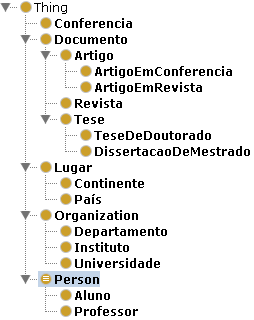
\includegraphics[width=7cm]{classes.png}
		\end{center}
		
	 

\end{document}


